%%%%%%%%% INTRODUCTION
% \section{Introduction}
\label{sec:01_intro}
\textit{``Does the text match the image?''} -- this simple question represents the Vision-and-Language Inference (VLI) task,
as shown in Figure~\ref{fig:example_vli}.
Image-text matching forms the backbone for V\&L pre-training~\citep{sun2019videobert,tan2019lxmert,lu2019vilbert,chen2020uniter} and has resulted in improvements in downstream tasks such as visual question answering, image retrieval, referring expressions, and visual commonsense reasoning.
While Natural Language Inference (without visual inputs) has been extensively studied~\citep{bowman2015large,williams2018broad,khot2018scitail,demszky2018transforming}, VLI demands the additional capability of being grounded in the scene while understanding semantics.
Although pre-trained language models (PLMs)~\citep{vaswani2017attention,devlin2019bert,raffel2020exploring} have been useful for encoding text into vector embeddings, recent findings point to undesirably high cosine similarity of two random words~\citep{ethayarajh2019contextual}, the struggle with negation~\citep{kassner2020negated,ettinger2020bert}, and semantically equivalent adversarial examples~\citep{ribeiro2018semantically}.
These findings call for robust training protocols to avoid propagation of these findings into VLI models.
\begin{figure}
    \centering
    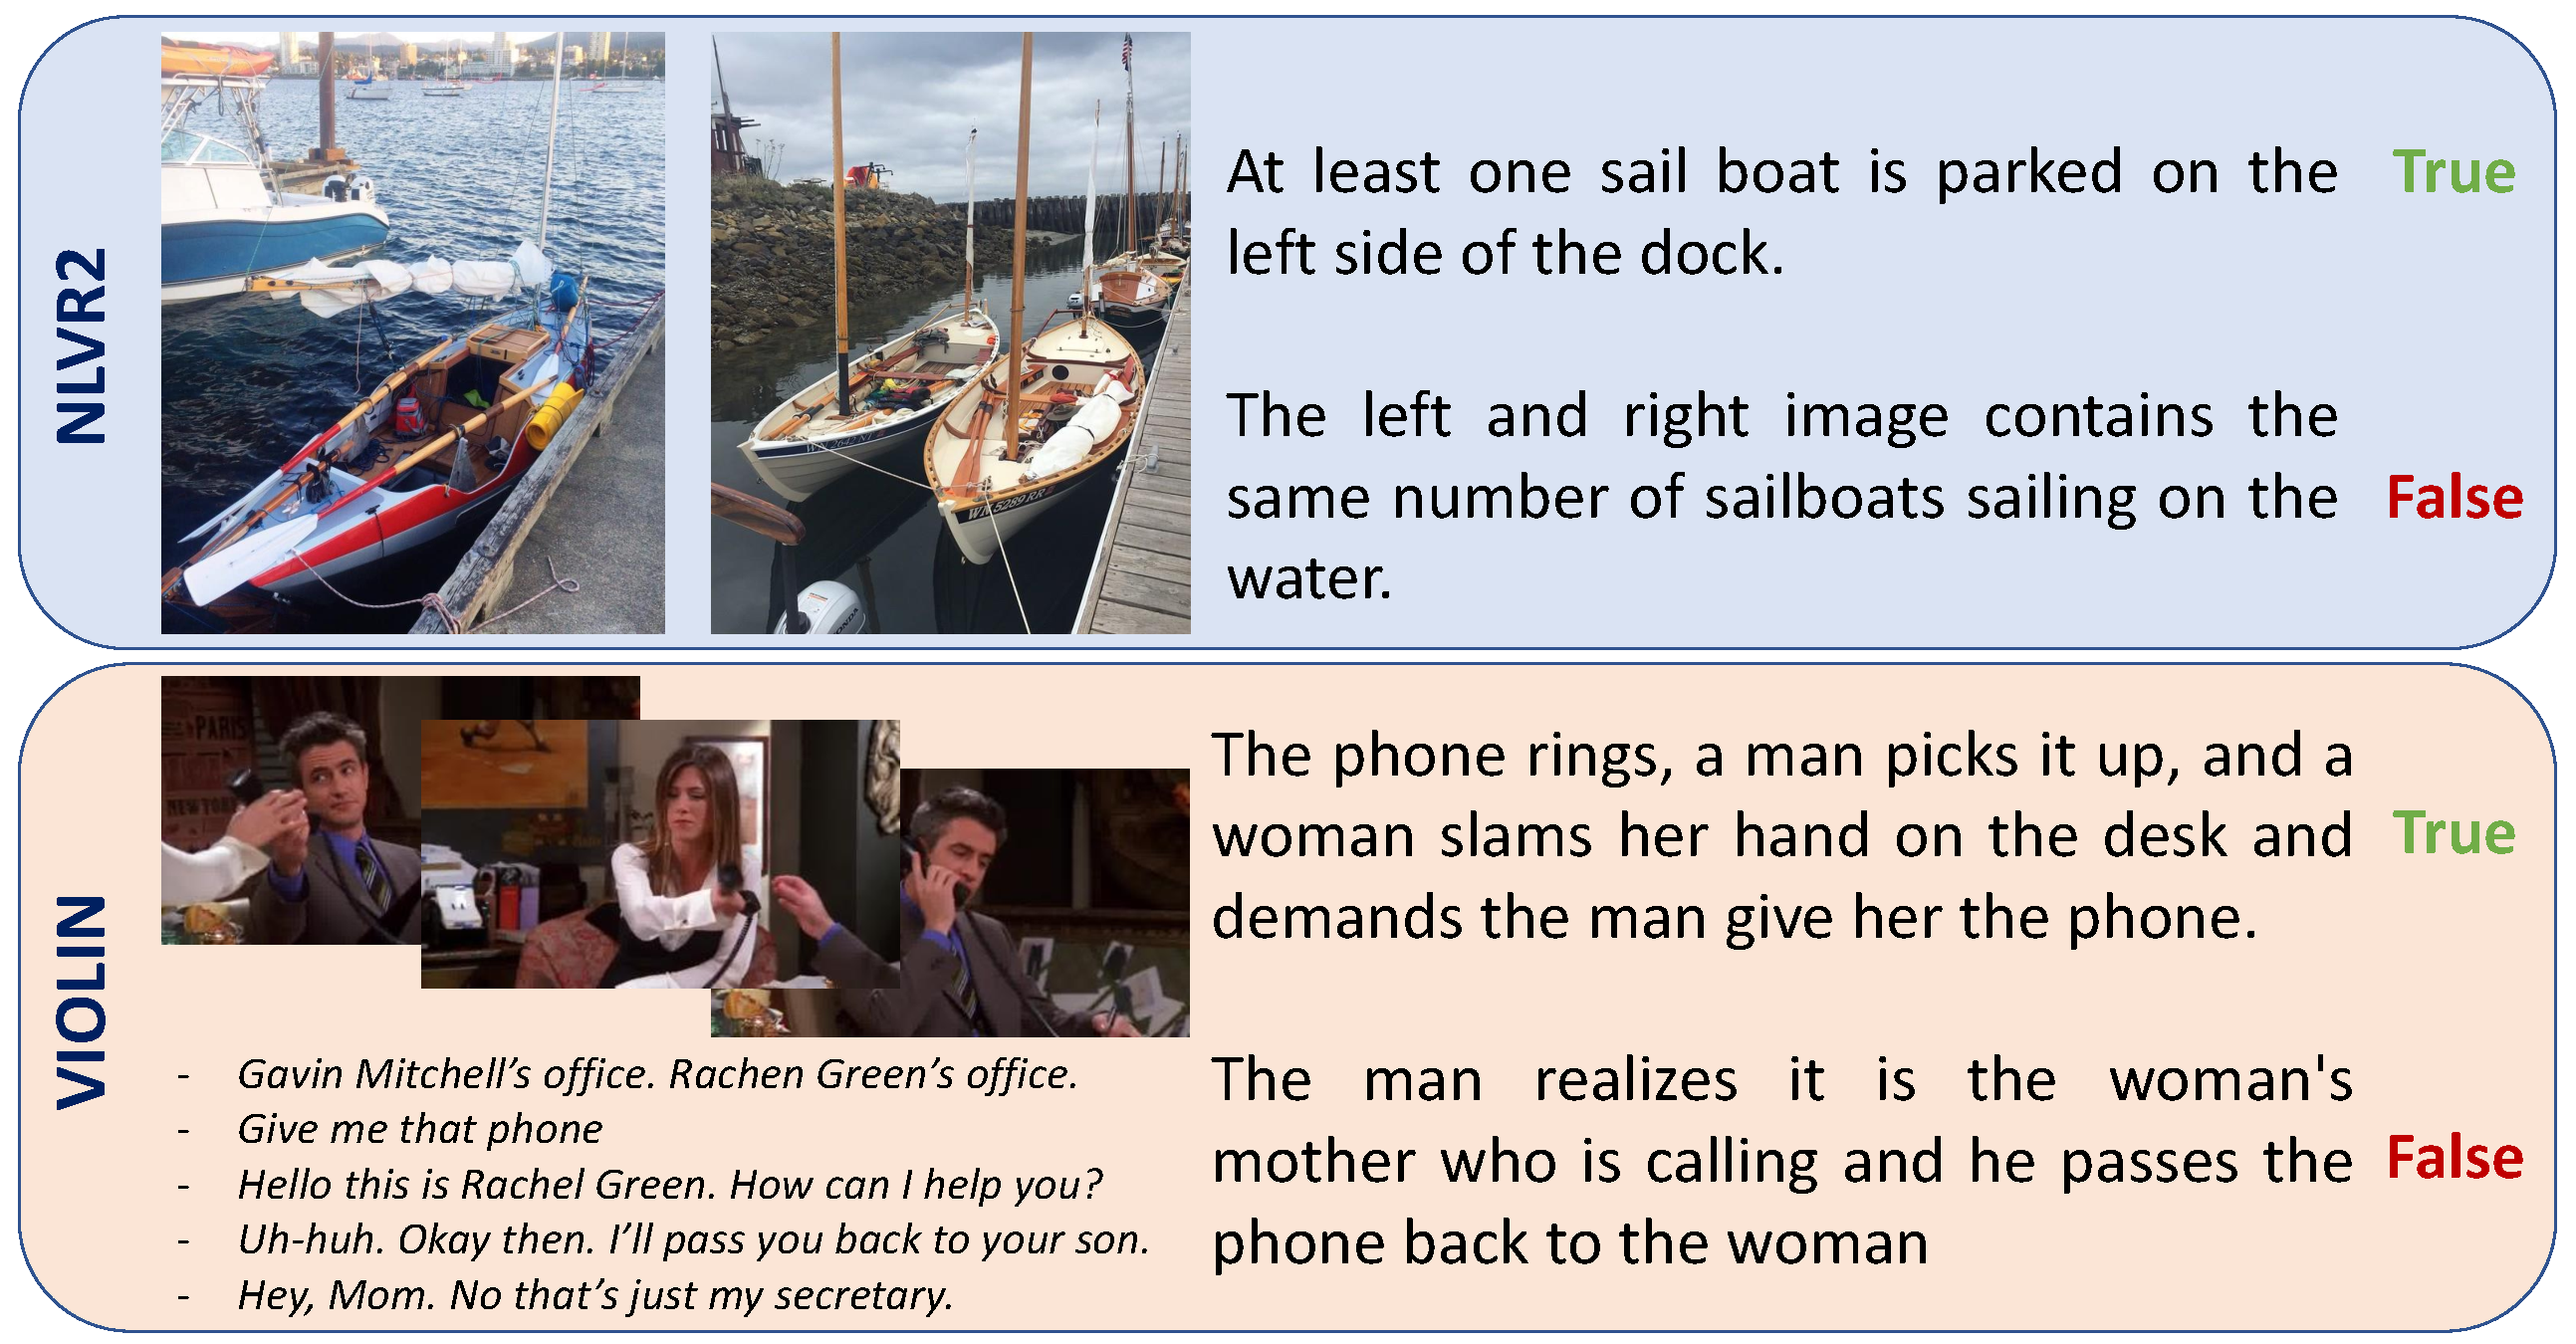
\includegraphics[width=\linewidth]{sdro/images/example_nlvr_violin.pdf}
    \caption{
        VLI models predict whether a sentence is \texttt{True} or \texttt{False} about the visual input. \textit{(Top)} sample from NLVR$^2$ with two images as input; \textit{(bottom)} sample from VIOLIN with video and subtitles as input.
        }
    \label{fig:example_vli}
\end{figure}


Adversarial training (AT) and distributed robust optimization (DRO)~\citep{madry2018towards,hu2018does,sinha2017certifying} have emerged as effective solutions to related problems in robust image classification, such as adversarial defense and domain generalization~\citep{volpi2018generalizing}.
DRO assumes a perturbation set (typically an $\ell_p$ norm ball) around the training distribution, and minimizes the worst-case performance over this perturbation set.
AT and DRO are popular for computer vision tasks, since the small perturbations of pixel intensities do not change the categorical meaning of the image.

However, in the case of text inputs, even small perturbations of their vector embeddings may result in absurd sentences or vectors that do not map to any word-token in vocabulary. 
The topology of the PLM embedding space is not well understood, especially with regard to what kind (and magnitude) of perturbations result in specific changes in semantics, such as similar meanings (speak $\rightarrow$ talk) or opposite meanings (Heaven $\rightarrow$ Hell) without resulting in random or absurd words.
We therefore argue that vector-based additive perturbations present limitations in the case of text inputs.
However, in the domain of natural language, we are blessed with semantic and logical transformations as shown in Table~\ref{tab:sisp_examples}.
This enables linguistically-informed perturbations with control over the semantics of the resulting sentence and label, as shown in Figure~\ref{fig:vector_vs_linguistic}.

\begin{figure}
    \centering
    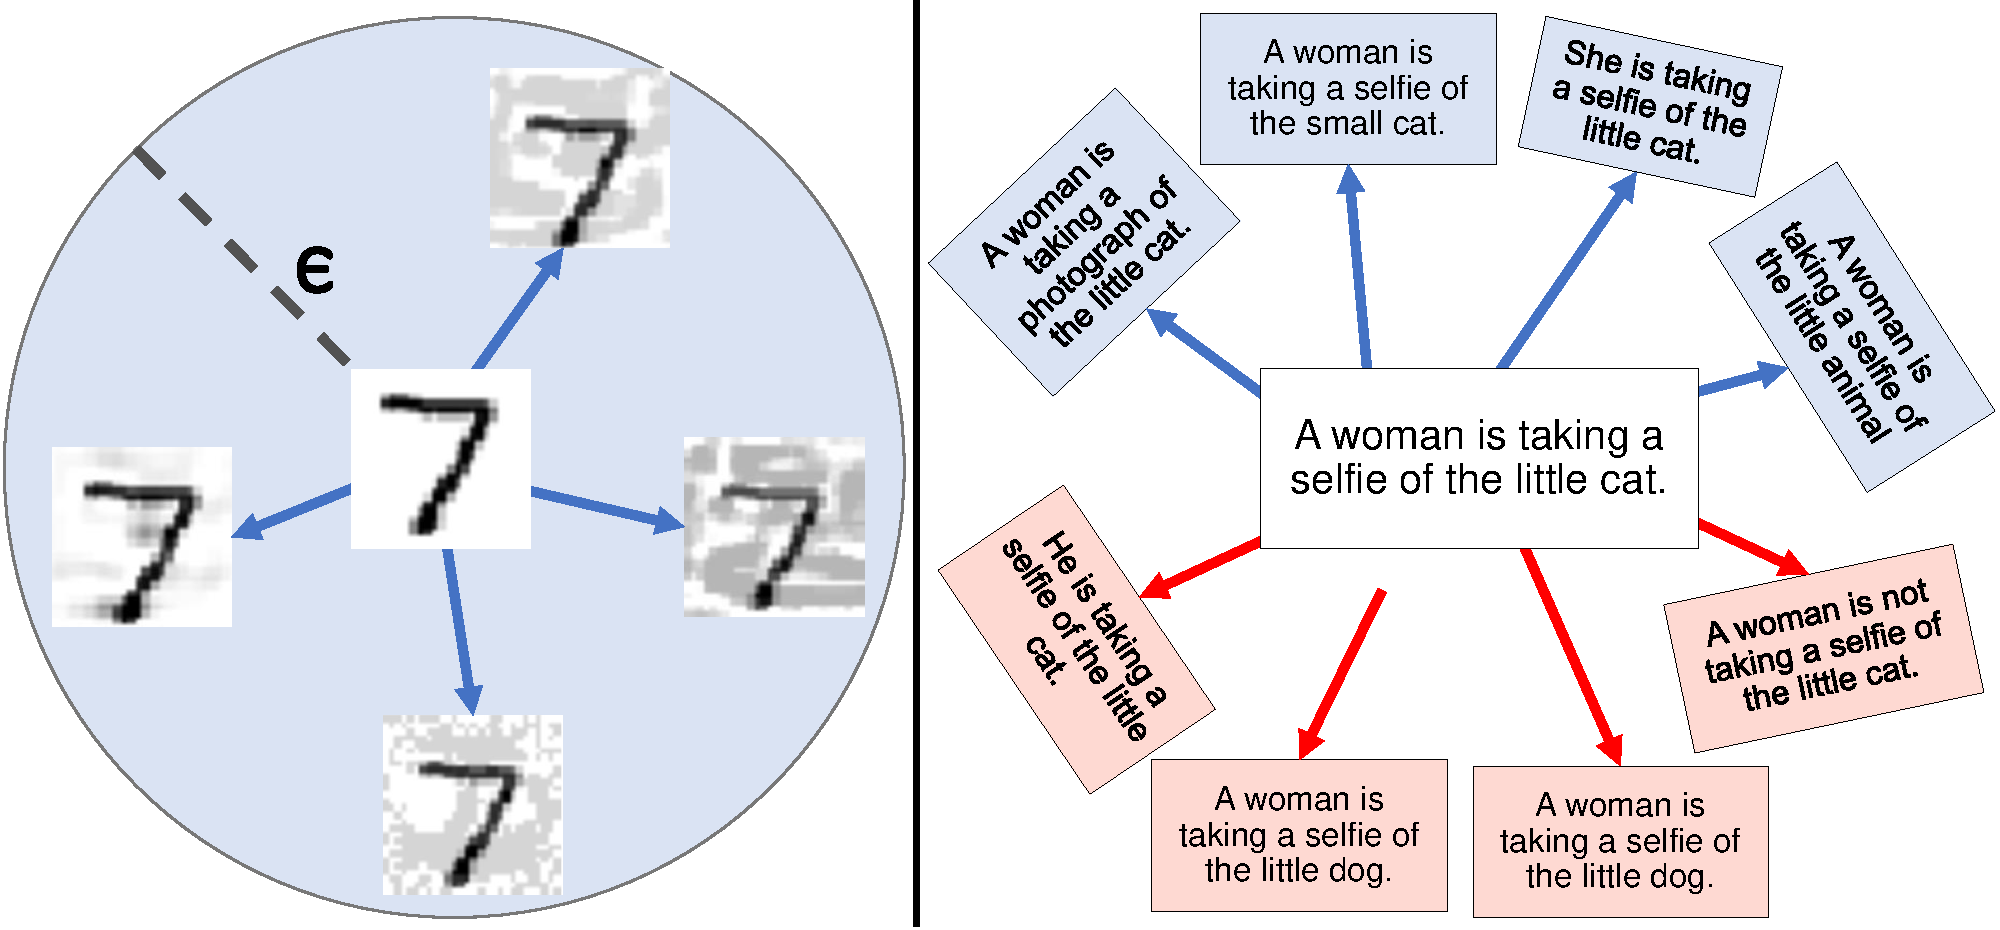
\includegraphics[width=0.95\linewidth]{sdro/images/vector_vs_linguistic.pdf}
    \caption{
    Comparison between \textit{(left)}
    \straightepsilon-bounded image perturbations and \textit{(right)} linguistics-based \textit{Semantics-preserving} (blue) as well as  \textit{Semantics-Inverting} (red) transformations for sentences.
    }
    \label{fig:vector_vs_linguistic}
\end{figure}
    
We present a technique that modifies robust optimization by incorporating linguistically-informed transformations.
Our approach: \textbf{S}emantically \textbf{D}istributed \textbf{R}obust \textbf{O}ptimization (SDRO) 
utilizes a pre-defined set of linguistic transformations (such as negation, word substitution, and paraphrasing) as the perturbation set instead of optimizing over the vector-space.
We dub this set of transformations ``SISP'' i.e., semantics-inverting (SI) and semantics-preserving (SP) transformations.
SDRO is \textit{model-agnostic} since it can be applied to text inputs of any existing VLI model and \textit{dataset agnostic} since it uses automated transformations without explicit knowledge of the text domain.

We apply SDRO to two VLI benchmark datasets: image-based NLVR$^2$~\citep{suhr2019corpus} as well as video-based VIOLIN~\citep{liu2020violin}.
To demonstrate the generalizability of SDRO to other V\&L tasks, we also report results on the ``yes/no'' subset of VQA-v2~\citep{goyal2017making}.
Our experiments show model-agnostic improvements in accuracy for all three benchmarks.
While models trained with naive data augmentation using SISP suffer from a trade-off between robustness and accuracy, models that utilize SDRO improve along both metrics.
SDRO also allows us to learn in low-resource settings, serving as a smart data augmentation tool -- SDRO models trained only with $80\%$ of the original dataset outperform existing state-of-the-art which utilizes the entire dataset.

Since SISP transforms do not require the true label to either produce an SP or SI transformed sentence, we can apply them at test-time.
Given a test input sentence, we generate its SISP versions and ensemble the predictions made by the model, giving equal weight to the prediction for the original sentence and the average predictions for all transformed sentences.
We find that this ensembling of predictions of the SDRO model at test-time pushes the state-of-the-art further, thereby demonstrating the usefulness of semantic sentence transformations, both during training and testing.
